\documentclass[11pt,a4paper,onecolumn,notitlepage]{article}
\usepackage[czech]{babel}
\usepackage[utf8]{inputenc}
\usepackage{lmodern}
\usepackage[T1]{fontenc}
\usepackage[text={17cm, 24cm},left=2cm,top=3cm]{geometry}
\usepackage{graphicx}
\usepackage{listings}
\usepackage{enumitem}
\usepackage[colorlinks]{hyperref}
\hypersetup{
	linkcolor = {black},
	citecolor = {black},
}

\providecommand{\uv}[1]{\quotedblbase #1\textquotedblleft}




\begin{document}
	\begin{center}
		\begin{figure}[hb]
			\centering
			
\includegraphics{FIT.eps}
			\label{fig:FIT}
		\end{figure}
	\vspace{\stretch{0.382}}
	\LARGE
		Mikroprocesorové a vestavěné systémy (IMP)\\
	\Huge
		Řízení modelů pomocí mikrokontroleru\\
	\vspace{\stretch{0.618}}
	\end{center}

{\Large v~Brně \hfill Václav Martinka\\
	\today \hfill xmarti76}

\pagenumbering{gobble}
\newpage

\tableofcontents

\newpage

\pagenumbering{arabic}

\section{Zadání}
Zvolte vhodný model (hotový, LEGO, Merkur nebo jiná stavebnice), který bude disponovat alespoň třemi různými funkcemi/pohyby funkčních bloků (např. bagr, jeřáb, robot apod.) Předpokládám, že zapojíte svoji tvořivost, aby výsledkem byl smysluplně vyhlížející a fungující celek.

Navrhněte vhodné rozhraní pro připojení pohybových elementů s FITkitem a vytvořte ovládací program v jazyku C pro MSP430, pomocí kterého bude možné interaktivně řídit všechny úkony modelu (pomocí příkazů zadávaných přes terminál s vhodně nastavenými parametry, případně prostřednictvím klávesnice FITkitu). Dále navrhněte alespoň dvě programové sekvence, na kterých budete demonstrovat činnost modelu realizujícího posloupnost zvolených povelů (jediným příkazem model vykoná složitější úkon).

	\subsection{Konkrétní řešení}
	Původně jsem měl v plánu ovládat plotr sestavený ze stavebnice merkur. Bohužel zde nastaly konstrukční problémy. Proto jsem se uchýlil k náhradnímu řešení - ovládání ventilátorů. Tedy možnosti jednotlivé ventilátory zapnout nebo vypnout včetně kontroly jejich funkčnosti.
	
	Využití tohoto systému si dokážu představit kdekoli, kde je potřeba chladit nějaké zařízení. Zejména v případě, že by se vstupy z klávesnice nahradili (nebo doplnili) vstupy z teplotních čidel.
	

\section{Návrh řešení}
Zadání obsahovalo několik bloků, které bylo nutné vyřešit. Ty jsou na sobě implementačně nezávislé, tudíž bylo možné je řešit postupně.
	
	\subsection{Spínání ventilátoru}
	Jelikož MCU není schopný na pinu dodat dostatečně vysoké napětí (12 V) ani proud (0,2 A) je nutné zapojení doplnit o spínací NPN tranzistor.
	\begin{figure}[hb]
		\centering
		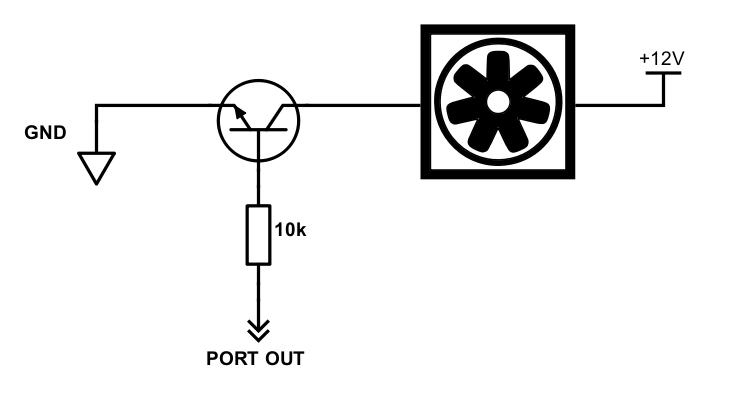
\includegraphics[width=0.9\textwidth]{fan.png}
		\caption{Schéma zapojení ventilátoru k MCU}
		\label{fig:fan}
	\end{figure}

	\subsection{Snímaní stavu ventilátoru}
	Pro projekt jsem využil 3vodičové ventilátory. Tedy takové, které kromě napájení obsahují ještě výstup z Hallovy sondy.
	\footnote{Hallova sonda je elektronická součástka, jejíž činnost je založena na technickém využití tzv. Hallova jevu. Používá se pro měření a automatickou regulaci magnetických polí, ovládání velkých elektromotorů, , bezkontaktní tlačítka, mechanické snímače (poloha, otáčky, zrychlení) apod. [\emph{zdroj Wikipedie (\url{https://cs.wikipedia.org/wiki/Hallova_sonda})}]}
	Na tomto vodiči se střídavě objevuje logická 0 a 1, podle toho, o kolik je otočena vrtule ventilátoru.
	Některé ventilátory vykazovali problémy, pokud byl tento vodič připojen přímo na vstup MCU. Bylo proto nutné jej přes rezistor (s hodnotou 10 k$\Omega$) připojit na napájení. Zároveň z důvodu ochrany MCU není vodič připojen přímo na vstup, ale je využit ještě předřadný rezistor.
	
	Signál z tohoto vodiče lze snadno využít pro kontrolu funkce ventilátoru -- pokud se hodnota nemění, tak se ventilátor zastavil. Taktéž by bylo možné tento signál využít pro měření otáček ventilátoru.

	\subsection{Vstup od uživatele}
	Jako uživatelský vstup jsem si vybral klávesnici a to zejména z důvodu jednoduchosti ovládání. V případě, že by zařízení mělo být ovládáno centrálně z nějakého vzdáleného místa, bylo by jistě vhodnější mít možnost zařízení ovládat i přes terminál.
	
	V reálném systému bych pak zařízení ještě doplnil o teploměry, aby bylo celé automatizované.
	
	
\section{Implementace}
Program pro MCU jsem implementoval v jazyce C. Vše je umístěno v jednom souboru a byli využity pouze standardní knihovny (\texttt{stdbool.h, fitkitlib.h, keyboard/keyboard.h, lcd/display.h}).

Základní inicializace je umístěna v těle funkce \texttt{fpga\_initialized()}. Ta se postará o nastavení logických vstupů/výstupů. Nastavení časovače a LCD.

Hlavní logika programu je pak umístěna v nekonečné smyčce ve funkci \texttt{main()}. Během této smyčky je obsloužena klávesnice, dojde ke kontrole, zda se ventilátory točí a vykreslení aktuálního stavu na LCD.

	\subsection{Kontrola ventilátorů}
	Nabízelo se několik řešení, jak tento problém vyřešit. Nakonec jsem se rozhodl pro přímočaré řešení. Načtu s odstupem 1 ms 8krát po sobě hodnotu ze vstupu, všech 8 hodnot si uložím do jednoho bytu. Pokud tento byte obsahuje 0xFF nebo 0x00, tedy samé 0 nebo 1, tak mám téměř jistotu, že se ventilátor netočí. Abych zaručil, že se otáčky ventilátoru neshodují s frekvencí MCU, tak během snímání provádím i jinou činnost (příprava hodnot pro vykreslení na LCD). Díky tomu vím, že hodnoty nejsou snímány pravidelně a je tudíž velmi malá šance, že nastanou falešná hlášení.
	
	\subsection{Vykonání programové sekvence}
	Při každém průchodu hlavní smyčky se volá funkce \texttt{running\_program()}. Ta je složena z přepínače \texttt{switch} s argumentem ID spuštěné sekvence.
	
	Na daném návěstí se nachází další \texttt{switch}, kde je jakožto argument čítač kroků sekvence. Tento čítač inkrementuji dle potřeby. Takto lze snadno napsat posloupnost jednotlivých kroků včetně podmínek, kdy se přechází na další krok. 
	
	
\newpage
\section{Popis chování}
Jak už jsem zmínil, zařízení se ovládá pomocí klávesnice:
\begin{description}[leftmargin=3em,style=nextline]
	\item[1 -- 9] Tyto klávesy slouží k zapnutí/vypnutí konkrétního ventilátoru. Protože program byl vytvořen jen pro tři ventilátory, jsou funkční pouze klávesy 1,2 a 3.
	\item[*] Tato klávesa sepne všechny ventilátory bez ohledu na jejich aktuální stav.
	\item[\#] Opak k *, tedy vypnutí všech ventilátorů.
	\item[A-D] Klávesy určené k sepnutí jednotlivých programových sekvencí. Jsou implementovány pouze 2~sekvence: A a B. Spuštění jedné ze sekvencí uzamkne klávesnici až do jejího vypnutí. Spuštěná sekvence je signalizována pomocí svítivé diody D5.
	\item[0] V případě, že je spuštěna nějaká sekvence, tak stisknutím dojde k vypnutí právě spuštěné sekvence, odemknutí klávesnice a zastavení všech ventilátorů.
\end{description}

	\subsection{Programové sekvence}
	\begin{description}[leftmargin=1.5em,style=nextline]
		\item[A] V této sekvenci se postupně spouští ventilátory 1, 2 a 3. Vždy po 7 sekundách, přičemž při sepnutí nového ventilátoru se ten předchozí vypne. Sekvence běží ve smyčce až do jejího ukončení.
		
		Využití by bylo v případě, že bychom potřebovali řídit velké (nebo velké množství) ventilátory s vysokým odběrem a přitom by nebyl vyžadován jejich stálý běh. V tom případě by bylo jistě vhodnější vždy spustit jen jeden, než střídavě zapínat/vypínat všechny naráz.
		
		\item[B] Tato sekvence se stará o bezpečné chlazení. Na začátku je spuštěn první ventilátor, v případě, že selže, dojde ke spuštění druhého. To se opakuje, dokud neselžou všechny ventilátory.
	\end{description}

	\subsection{Výstup na LCD}
	Po celou dobu běhu programu je na LCD zobrazován aktuální stav všech ventilátorů. Ten nabývá tří hodnot:
	\begin{description}[leftmargin=3em,style=nextline]
		\item[OFF] Značí vypnutý ventilátor
		\item[OK] Ventilátor je zapnutý a nehlásí žádné problémy
		\item[ERR] Došlo k chybě ventilátoru
	\end{description}
	
	
\section{Závěr}
I přes prvotní problémy s plotrem se mi nakonec podařilo vytvořit funkční zařízení. Výsledný kód by měl být poměrně snadno rozšířitelný na větší množství ventilátorů, což byl jeden z mých cílů.

Co se týče možnosti rozšířitelnosti do budoucnu, tak by to bylo doplnění snímání počtu otáček, řízení rychlosti otáček (to vyžaduje jiné ventilátory) nebo přidání teploměrů.

\end{document}          
